\section{Two literatures, measured}
\label{sec:literatures}

Section~\ref{sec:taxonomy} shows the two communities working on one problem
space. This section asks whether they are aware of each other. We measure it
twice, first by citation and then by evaluation. The second measurement is much
worse than the first.

\subsection{Citation}

We compute cross-track citation over the whole coded population, the
\NTrackSecurity{} security and \NTrackML{} machine learning papers that
classify into one track, not over a sample. A
paper counts as citing the other track if it cites any paper anywhere in the
discovery pool that resolves to that track.

\begin{itemize}
\item \textbf{\PctSecCitesML{}\%} of security papers (\NSecCitesML{} of
  \NTrackSecurity{}) cite at least one machine
  learning paper on the same failure.
\item \textbf{\PctMLCitesSec{}\%} of machine learning papers (\NMLCitesSec{} of
  \NTrackML{}) cite at least one
  security paper.
\end{itemize}

Figure~\ref{fig:network} shows the same corpus as a graph. Because these are
population counts rather than sample estimates, no confidence interval
applies. Roughly nine papers in ten, on both sides, were written
without reference to the other community's work on the same failure.

The rates are stable across evidence grade, so this is not an artifact of
preprint quality. Peer-reviewed security papers cite the other track 15.1\% of
the time against 11.1\% for preprints, and the machine learning side is flat at
8.6\% against 9.5\%.

\textbf{What carries the cross-track citations makes the rate look better than
the engagement is.} \NNetworkCross{} of the \NNetworkEdges{} resolved edges
(\PctNetworkCross{}\%) cross tracks, and they run through 333 papers, but they are concentrated: the ten most-cited
bridge papers account for 27\% of all cross-track edge endpoints. Those ten are
not method papers engaging with the other community's methods. They are
surveys, benchmarks and canonical references: a cross-literature threat survey,
WebArena, AgentDojo~\cite{debenedetti-2024-agentdojo}, InjecAgent,
\emph{Lost in the Middle}~\cite{liu-2023-lost}, and
PoisonedRAG~\cite{zou-2024-poisonedrag}. A security paper that cites
\emph{Lost in the Middle} in passing is scored as citing the other track, and
by our measurement it does. It has not thereby engaged with the machine
learning literature's methods. \textbf{The \PctSecCitesML{}\% and \PctMLCitesSec{}\% are therefore upper bounds on engagement,
not estimates of it},, which is the second reason the
evaluation measurement below matters more than the citation one.

\begin{figure}[t]
\centering
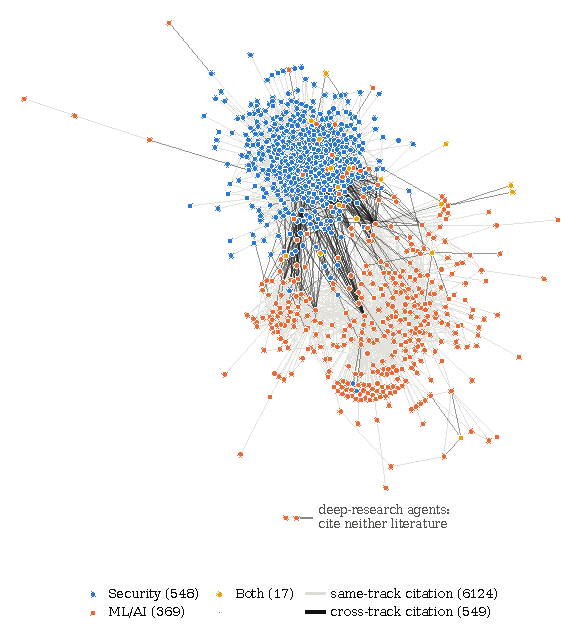
\includegraphics[width=\columnwidth]{figures/fig5_citation_network}
\caption{The corpus as a citation graph: \NNetworkNodes{} papers that cite or are cited
by another included paper, \NNetworkEdges{} edges. Node colour is track. Pale edges are
citations within one literature, dark edges cross between them. The two
communities form separate clusters joined by a narrow band. Note that 8.2\% of
\emph{edges} cross tracks, which is not the same measurement as the per-paper
rates in the text: a paper counts there if it has at least one cross-track
citation anywhere in its reference list. Papers with no resolved citation link to any other
included paper are omitted from the drawing.}
\label{fig:network}
\end{figure}

\subsection{Evaluation}

Citation is a weak test. A paper can cite a neighbouring literature in one line
of related work and ignore it everywhere else. The stronger test is whether a
defense is ever \emph{evaluated} against a mechanism from the other track.

Of the confirmed defense-by-mechanism test pairs in our coverage matrix,
\textbf{230 of 232 (99.1\%) stay inside a single track. Two cross it, and only
one is a genuine cross-community test.}

This is roughly an order of magnitude worse than the citation gap. The two
literatures cite each other rarely. They evaluate against each other's problems
almost never.

\subsection{What the split costs}

Three consequences follow, and all three are visible in the numbers.

\textbf{Named problems go unanswered.} \NMechUncovered{} of
\NMechanismsBench{} named mechanisms (\PctMechUncovered{}\%) have no defense
ever evaluated against them. Among named injection variants,
\NInjUncovered{} of \NInjVariants{} have zero tested defenses, while the single umbrella entry "indirect
prompt injection" absorbs 76 pairs, which is 32.6\% of all pairs in the matrix.
The field tests heavily against a category and lightly against its members.

\textbf{Effort concentrates where it is already dense.} The incidental half has
4.6 defenses per failure mode and the adversarial half has 1.4 per attack, as
Section~\ref{sec:taxonomy} reports. A community that does not read the other
one cannot see that it is crowding.

\textbf{Methods are adopted without a worst-case check.} \PctOneThreatModel{}\% of defenses were
validated against one threat model. For the \NIncOnly{} validated only on incidental
benchmarks, no one has asked what an adversary does to them. That question is
what Section~\ref{sec:experiments} answers for a sample of them.
